\documentclass[a4paper,oneside,11pt]{book}

\usepackage{amsbsy}
\usepackage{amsmath}
\usepackage{amsfonts}
\usepackage{graphicx}
\usepackage{multirow}
\usepackage{mathrsfs}
\usepackage{xcolor}
\usepackage[hidelinks]{hyperref}
\usepackage{enumitem}
\usepackage{epsfig}
\usepackage{caption}
\usepackage{subcaption}
\usepackage{booktabs}
\usepackage{tabularx}
\usepackage{array}
\usepackage{rotating}
\usepackage{float}
\usepackage{placeins}
\usepackage[strict]{changepage}

% Page Margins - Strath Requirement
\usepackage[left=4cm,right=2.5cm,top=2cm,bottom=4cm,includehead,includefoot,headheight=15pt]{geometry}

% Page Headers
\usepackage{fancyhdr}
\fancyhf{}
\renewcommand{\headrulewidth}{0pt} % optional
%\fancyhead[L]{\nouppercase{\leftmark} \hfill Section \nouppercase{\rightmark}}
\fancyhead[L]{\nouppercase{\leftmark}}
\cfoot{\thepage}
\pagestyle{fancy}

% Line Spacing
%\def\baselinestretch{1.5} 
\usepackage{setspace}
\setstretch{1.5}

% Place UoS Logo on Title Page (this package modifies the "\maketitle" command.)
\usepackage{titling}
\pretitle{%
  \begin{flushright}
  \vspace{-9.5cm}
  
\includegraphics[width=5cm]{strathlogo.jpg} \\[7cm]
  \end{flushright}
  \begin{center}
  \LARGE
}
\posttitle{\end{center}}

  \title{CS818 Assessment\\Factors impacting obesity rates\\[1ex]
  \small Word count (from TexCount): 3241}
\usepackage[backend=biber]{biblatex}
\addbibresource{/home/joebutler/Documents/Msc/CS818/assessment/CS818_obesity.bib}

%%%%%%%%%%%%%%%%%%%%%%%%%%%%%%%%%%%%%%%%%%%%%%%%%%%%%%%%%%%%%%
\begin{document}
\maketitle


%%%%%%%%%%%%%%%%%%%%%%%%%%%%%%%%%%%%%%%%%%%%%%%%%%%%%%%%%%%%%%
\frontmatter
%%%%%%%%%%%%%%%%%%%%%%%%%%%%%%%%%%%%%%%%%%%%%%%%%%%%%%%%%%%%%%

\tableofcontents

\addcontentsline{toc}{chapter}{List of Figures}
\listoffigures

\addcontentsline{toc}{chapter}{List of Tables}
\listoftables

%%%%%%%%%%%%%%%%%%%%%%%%%%%%%%%%%%%%%%%%%%%%%%%%%%%%%%%%%%%%%%
\mainmatter
%%%%%%%%%%%%%%%%%%%%%%%%%%%%%%%%%%%%%%%%%%%%%%%%%%%%%%%%%%%%%%

\chapter{Introduction}
%!TEX root = CS818_assessment.tex
Obesity is a critical public health challenge, with links to elevated risk of type 2 diabetes, cardiovascular disease, and certain cancers \cite{Kinlen2018}. Epidemiological research has long established that lifestyle factors - most notably diet and physical activity — are closely associated with body mass index (BMI) and general metabolic health \cite{Bergens2020}. These factors subsequently form the basis of much public health advice on obesity. However, the strength and nature of these associations can be heterogeneous across different populations. For example physically active and metabolically healthy individuals may nevertheless be obese \cite{Alcazar2021}, and this combination is more prevalent amongst females and younger age groups \cite{Bluher2020}. Similarly, whilst a diet rich in saturated fats has been linked to increased obesity risk \cite{Wang2020}, countries like France maintain comparatively low levels of obesity with comparatively high saturated fat intake \cite{Ducrot2018}.

This heterogeneity presents a challenge for public health officials seeking to identify the most impactful interventions. It also challenges conventional statistical methods, which often assume homogenous relationships between variables \cite{Hoekstra2012}. More advanced analytical techniques are required to disentangle these complex relationships between lifestyle factors and obesity.

This study adds to the debate by exploring the multifactorial nature of obesity with both supervised and unsupervised learning techniques. The findings highlight key lifestyle factors associated with obesity as well as their interrelationships, which may permit more targeted public health interventions.


\chapter{Data}
%!TEX root = CS818_assessment.tex
\section{Overview of dataset}
The analysis in this study is based on a dataset from the UC Irvine Machine Learning Repository \cite{Obesity}, comprising 2111 observations across 17 variables collected from participants in Mexico, Peru and Colombia. Approximately 77\% of the data is synthetic, which was used to address an unbalanced distribution in obesity levels \cite{Palechor2019a}. The target variable is obesity level, labelled 'NObeyesdad' in the dataset. This categorises individuals based on their BMI into the groups Insufficient Weight, Normal Weight, Overweight Level I, Overweight Level II, Obesity Type I, Obesity Type II and Obesity Type III. The calculation for BMI is
\[
\text{BMI} = \frac{\text{Weight (kg)}}{(\text{Height (m)})^2}
\]
and obesity is defined as a BMI equal or greater to 30.00 in line with the World Health Organisation's definition \cite{Palechor2019a}. The coded variables that appear in the dataset are detailed in table \ref{tab:variables}.

\begin{table}[!h]
\centering
\begin{tabular}{|l|l|}
\hline
\textbf{Variable Name} & \textbf{Description} \\
\hline
family\_history\_with\_overweight & Family history of overweight \\
FAVC & Frequent consumption of high-caloric food \\
FCVC & Frequency of vegetable consumption in meals \\
NCP & Number of main meals per day \\
CAEC & Frequency of food consumption between meals \\
SMOKE & Smoking status \\
CH2O & Daily water consumption \\
SCC & Monitoring of daily calorie intake \\
FAF & Frequency of physical activity \\
TUE & Daily usage time of technological devices \\
CALC & Frequency of alcohol consumption \\
MTRANS & Usual mode of transportation \\
NObeyesdad & Obesity level \\
\hline
\end{tabular}
\caption{Variables and Descriptions}
\label{tab:variables}
\end{table}

\section{Exploratory analysis: results}

Figure \ref{fig:distributions} captures the distribution of the demographic variables, which shows a right-skew for age with a mean of 24.3 years and few entries from participants aged 40 and above. This could limit how well any findings generalise to older populations. Weight's distribution is unimodal and slightly right-skewed, with a mean of 86kg, whilst height's distribution is more symmetrical, with a mean of 1.7m.

\begin{figure}
  \centering
  \begin{subfigure}[b]{0.7\textwidth}
    \centering
    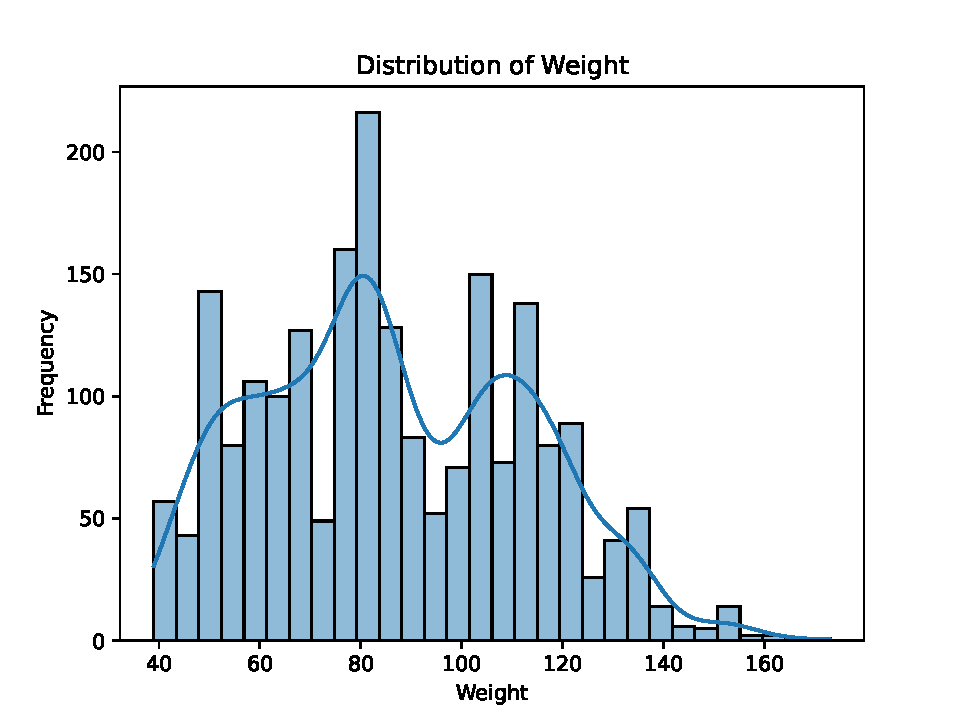
\includegraphics[width=\textwidth]{weight_dist.pdf}
    \label{fig:weight}
  \end{subfigure}
  \hfill
  \begin{subfigure}[b]{0.7\textwidth}
    \centering
    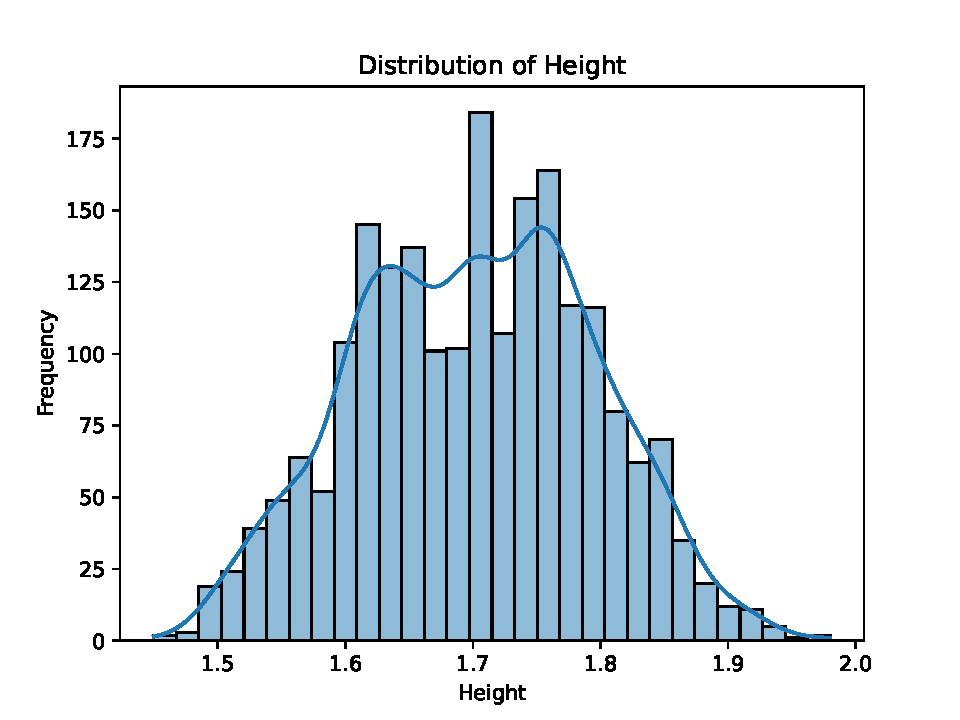
\includegraphics[width=\textwidth]{height_dist.pdf}
    \label{fig:height}
  \end{subfigure}
  \hfill
  \begin{subfigure}[b]{0.7\textwidth}
    \centering
    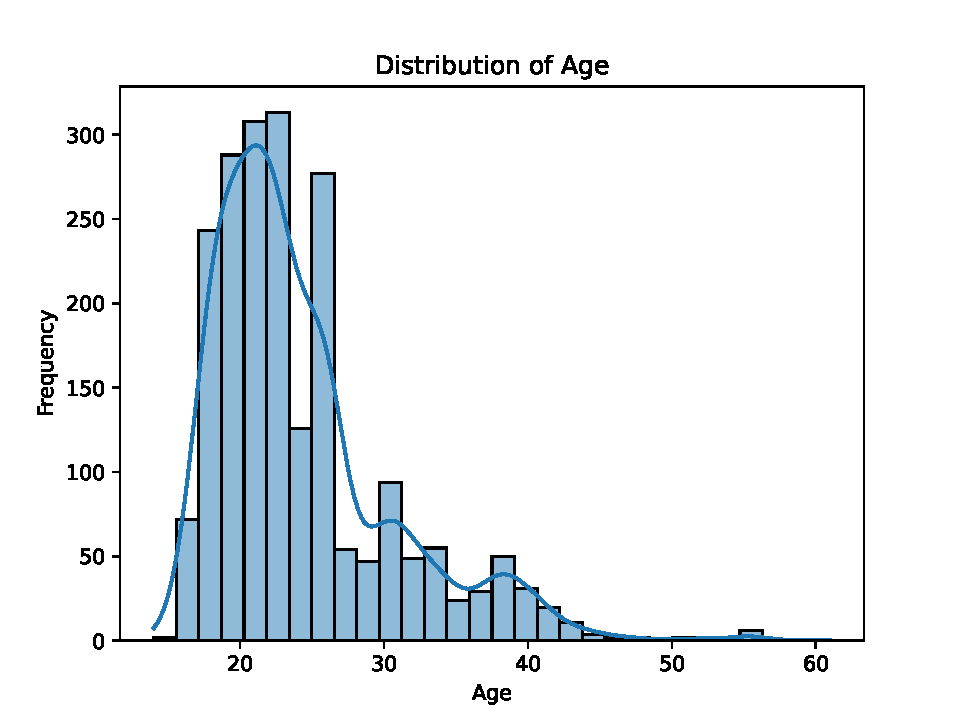
\includegraphics[width=\textwidth]{age_dist.pdf}
    \label{fig:age}
  \end{subfigure}
  \caption{Distributions of weight, height, and age.}
  \label{fig:distributions}
\end{figure}

Expanding out the exploratory analysis, we can consider the correlation between numeric variables. To ensure obesity rate is captured, the category 'BMI' will be added using the formula already given. And since BMI is calculated from height and weight, those categories will be removed to avoid duplication and to focus in on variables beyond body-measurements.

\begin{figure}
  \centering
  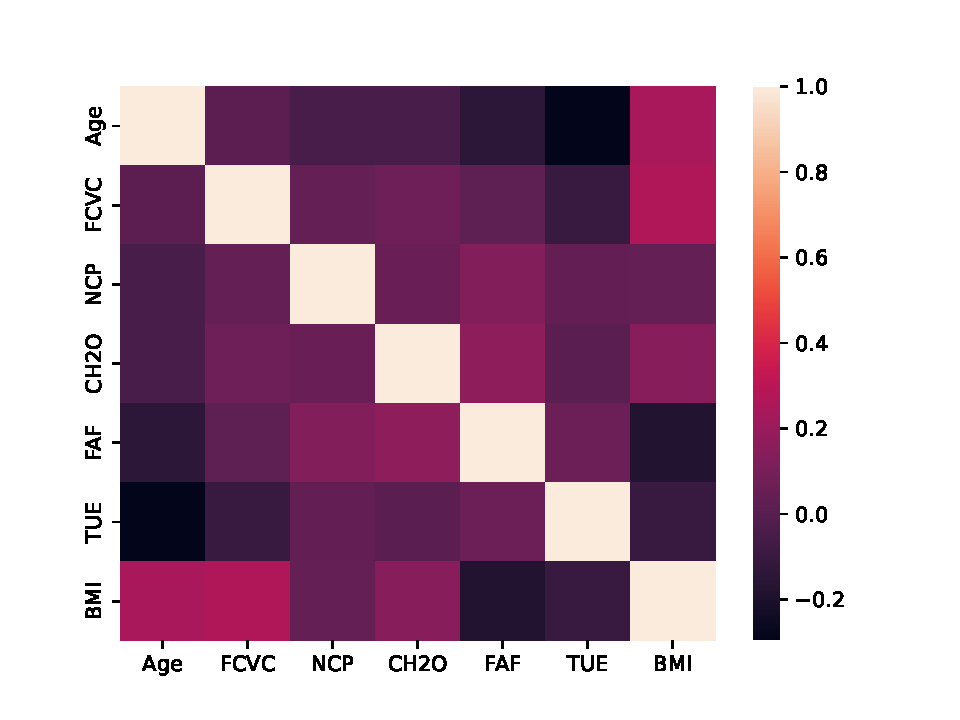
\includegraphics[width=0.8\textwidth]{numeric_correlations.pdf}
  \caption{Correlation Heatmap}
  \label{fig:heatmap}
\end{figure}

\begin{table}
\centering
\caption{Strongest Correlation Pairs}
\label{tab:top_correlations}
\begin{tabular}{llr}
\toprule
Variable 1 & Variable 2 &  Correlation \\
\midrule
Age        & TUE        &    -0.297 \\
BMI        & FCVC       &     0.264 \\
Age        & BMI        &     0.244 \\
BMI        & FAF        &    -0.178 \\
CH2O       & FAF        &     0.167 \\
Age        & FAF        &    -0.145 \\
BMI        & CH2O       &     0.144 \\
FAF        & NCP        &     0.130 \\
FCVC       & TUE        &    -0.101 \\
BMI        & TUE        &    -0.100 \\
\bottomrule
\end{tabular}
\end{table}

As per figure \ref{fig:heatmap} and table \ref{tab:top_correlations}, the strongest correlation is the negative relationship between age and time on electronic devices, though this relationship is not directly applicable to obesity. Of greater relevance are positive relationships between BMI and both vegetable consumption (FCVC) and age. There is also a negative relationship between BMI and physical activity (FAF), though in all cases the strength of the relationship is fairly weak. 

\FloatBarrier

The dataset also contains the categorical variables CALC (how often a respondent drinks alcohol) and CAEC (how frequently a respondent eats between meals). In both cases, the data is heavily concentrated in the 'Sometimes' category, though there were a reasonable number of respondents who noted they never drink alcohol, as per \ref{fig:calc_caec}. Similarly, the MTRANS (mode of transport) variable in figure \ref{fig:MTRANS_heatmap} shows the vast majority of respondents travelling by public transport, with a smaller minority travelling by automobile, and very few travelling by either bike, motorbike, or walking. In their current skewed form, these variables could disproportionately influence model estimates or clustering outcomes.

\begin{figure}
  \centering
  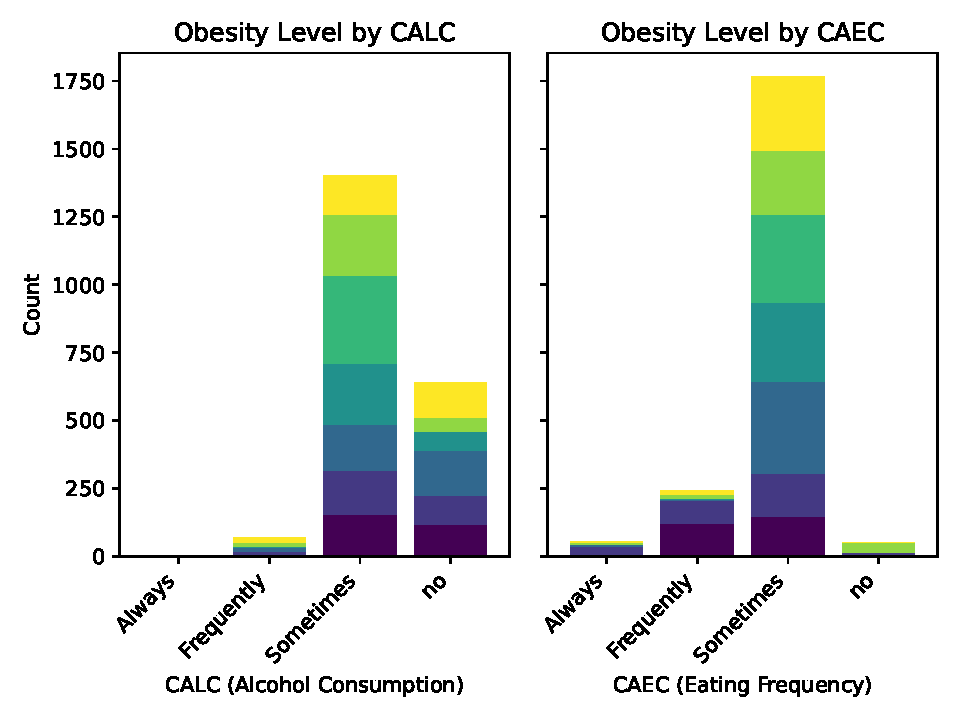
\includegraphics[width=0.8\textwidth]{CALC_and_CAEC.pdf}
  \caption{Distribution of Obesity Level by CALC and CAEC}
  \label{fig:calc_caec}
\end{figure}


For the final section of this exploratory analysis, we can consider how the binary variables relate to obesity levels. Here, 'Obese' follows the WHO definition as falling in category Obesity Type I, II and III, whilst 'Not obese' is all remaining categories, representing a BMI of below 30. As shown in figure \ref{fig:binary_obesity}, whilst an individual's gender or smoking status has little relation to obesity levels, individuals reporting a family history of obesity are significantly more likely to be obese than those with no such family history. Similarly, high consumption of calorific foods (FAVC) is perhaps unsurprisingly associated with higher obesity, and monitoring calories with lower obesity.   

\begin{figure}
  \centering
  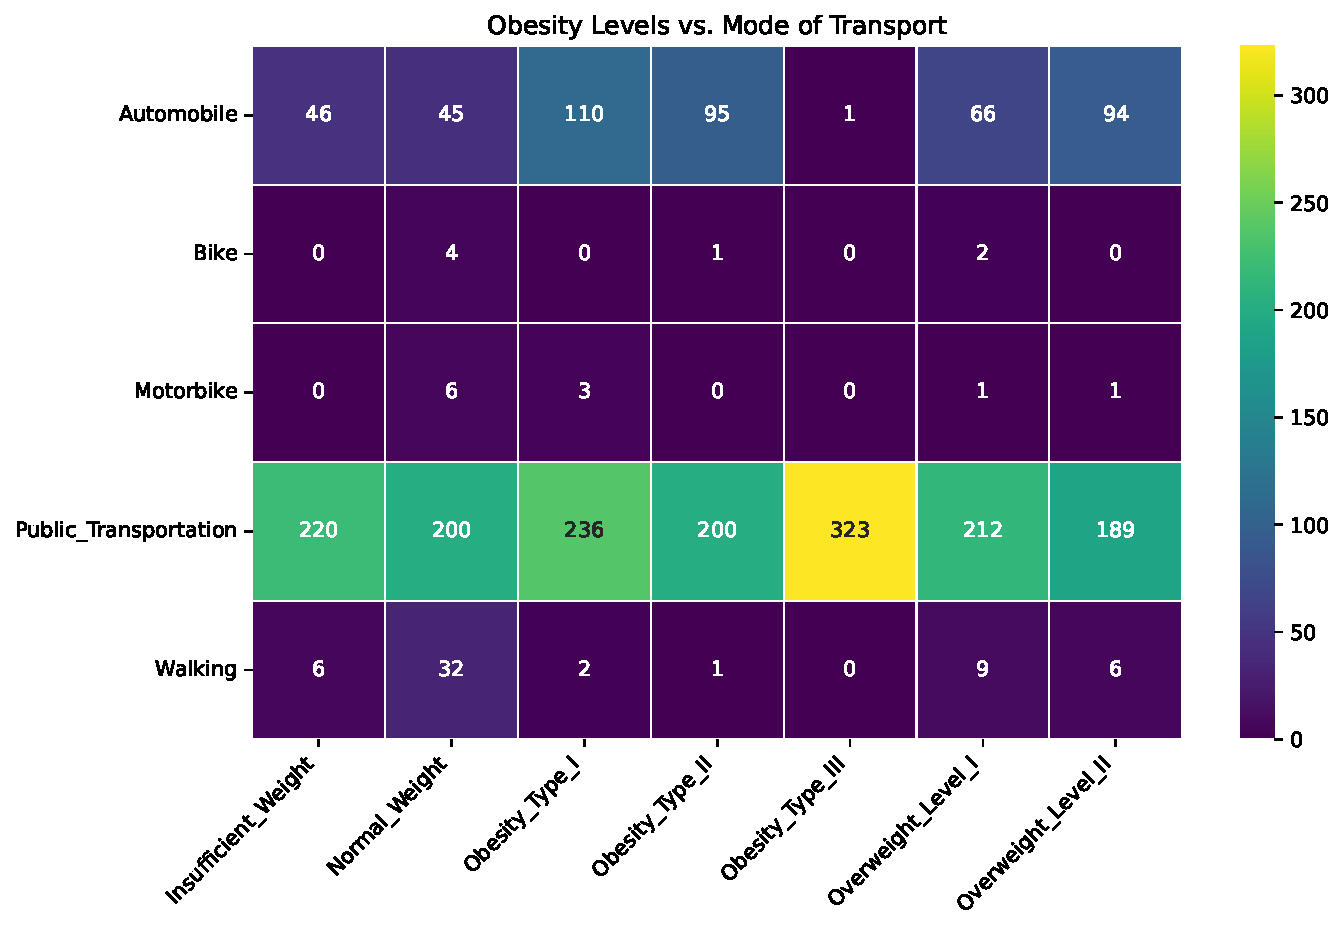
\includegraphics[width=1\textwidth]{MTRANS_heatmap.pdf}
  \caption{Obesity Levels vs. Mode of Transport}
  \label{fig:MTRANS_heatmap}
\end{figure}

\begin{figure}
  \centering
  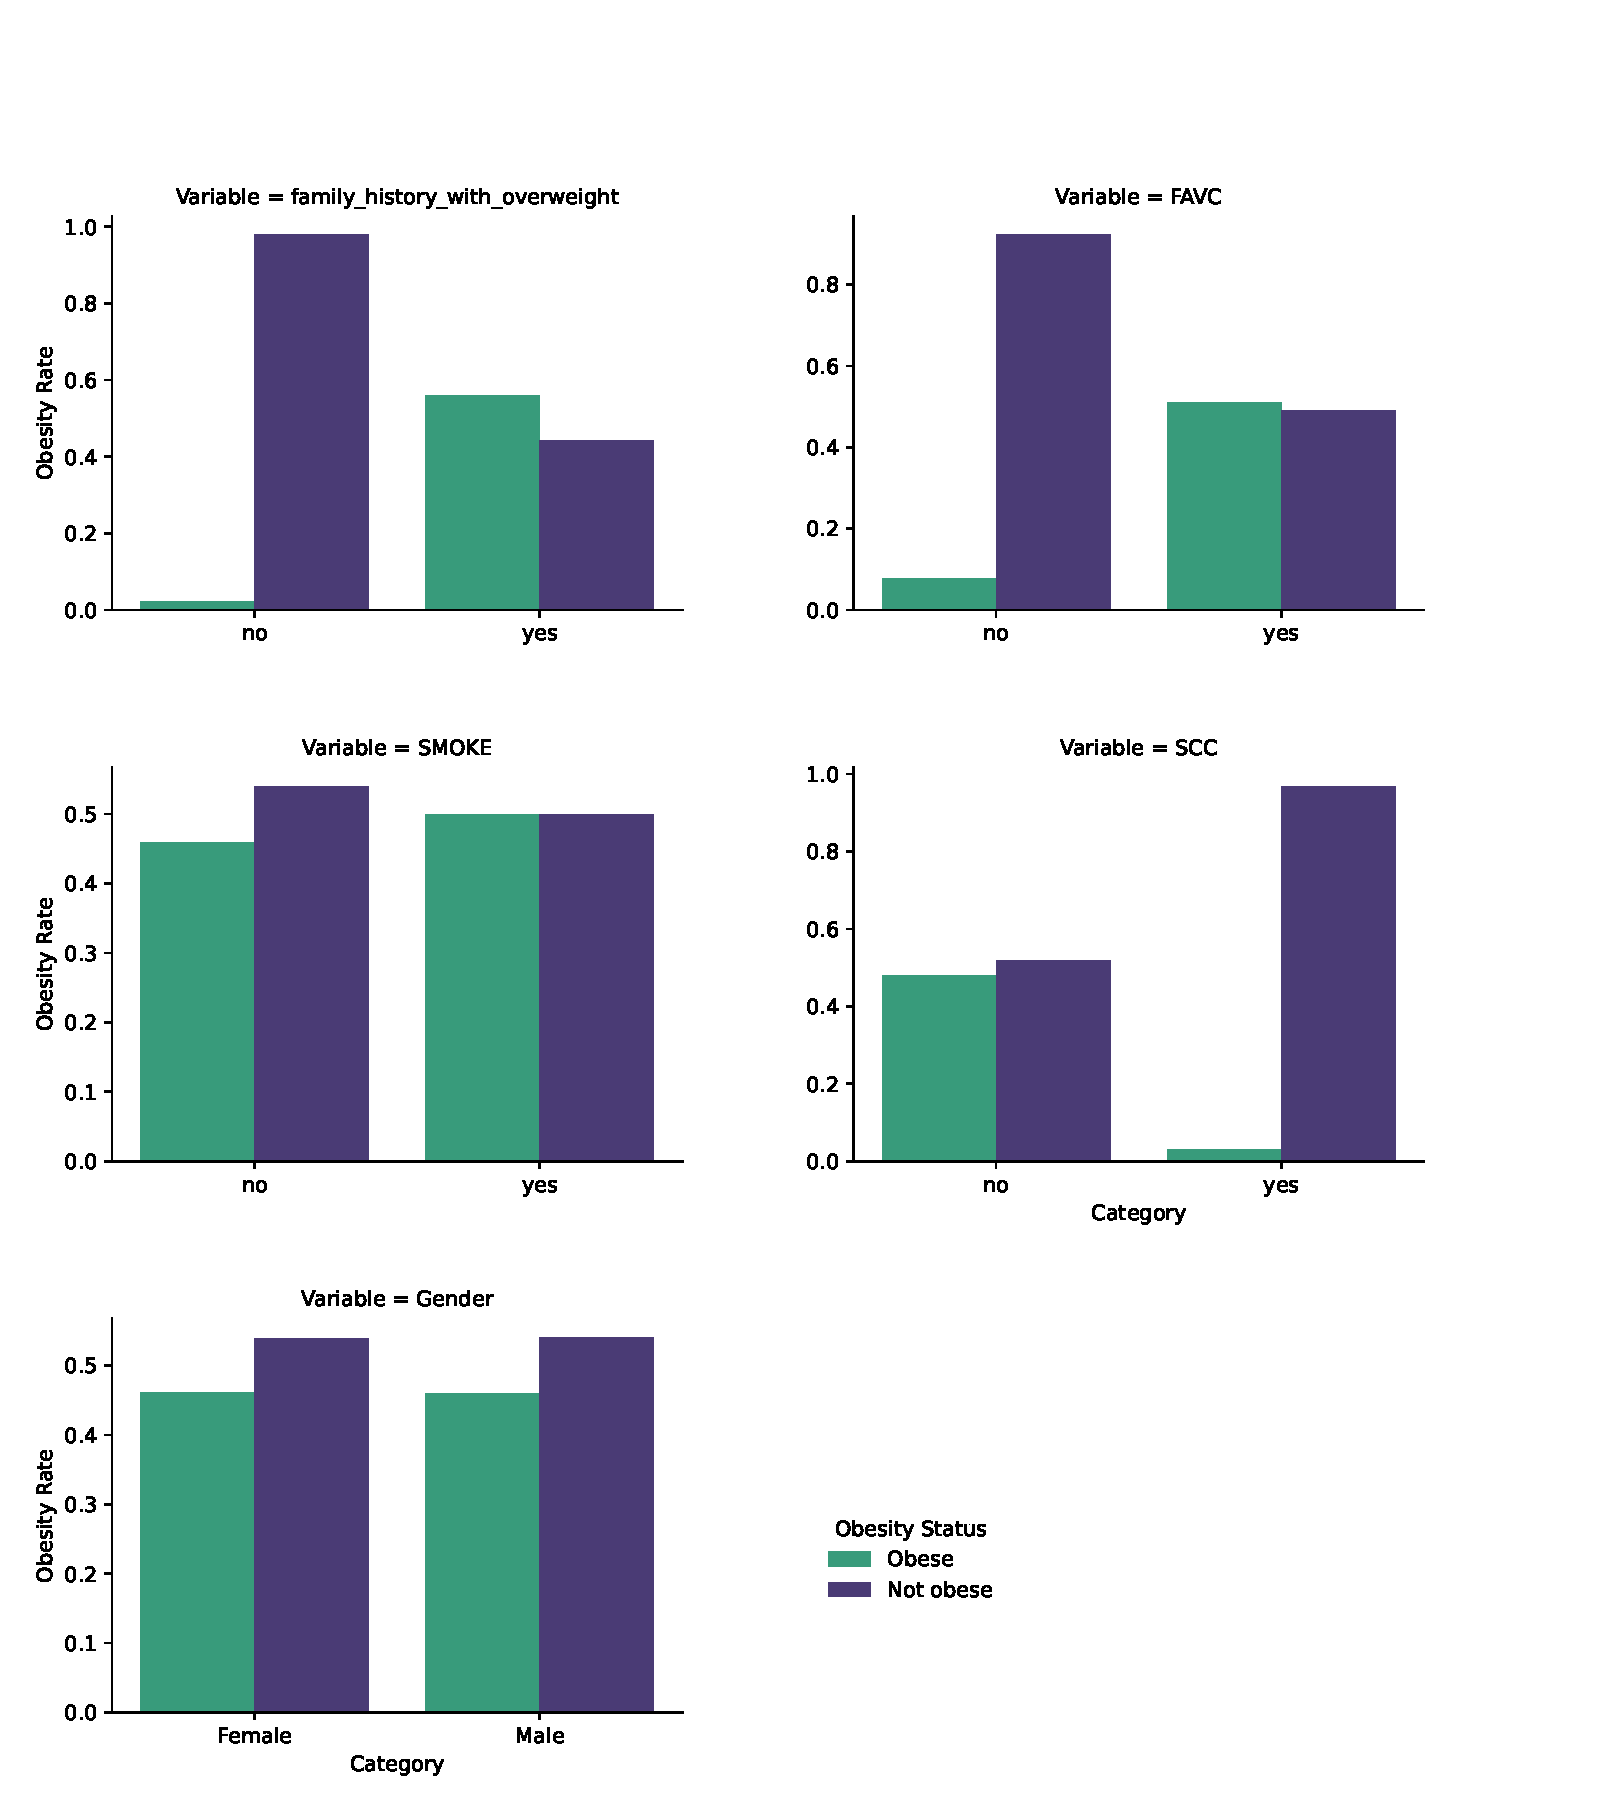
\includegraphics[width=1\textwidth]{binary_obesity.pdf}
  \caption{Obese vs. Not Obese for Binary Variables}
  \label{fig:binary_obesity}
\end{figure}

\FloatBarrier
\section{Discussion}

This initial exploratory analysis has provided a clear understanding of the dataset. Bivariate analysis was used to identify correlations. The link between low physical activity and higher BMI is consistent with research showing the positive impact exercise has on obesity risk \cite{Bergens2020}. Similarly, individuals may become more sedentary as they grow older, which could contribute to the link between age and BMI. However, the fact that higher vegetable consumption is correlated to higher BMI directly contradicts findings and public health advice which encourages greater vegetable consumption as a means of reducing obesity risk \cite{Nour2018}. This will be considered when conducting further analysis in the report's remaining sections. Similarly, analysis highlighted the concentration of responses to certain categorical variables such as alcohol consumption, which could indicate a predisposition amongst respondents towards particular behavioural patterns which will be borne in mind. Finally, the dataset is primarily made up of synthetic data. Whilst the SMOTE technique used by the creators is methodologically robust, there is always a risk with synthetic data that it fails to capture real-world variability \cite{Giuffre2023}. These potential limitations will be considered when evaluating the generalisability of any findings.

Whilst this approach has allowed us to uncover trends, univariate and bivariate analysis does not adequately capture the interactions between variables. For example, the correlation matrix shows a strong correlation between age and time on electronic devices, and separately between age and BMI, suggesting but leaving unexplored an interplay between these factors. To better understand potential interrelationships, more advanced multivariate techniques must be employed, which is the subject of the following section. 



\chapter{Unsupervised Analysis}
%!TEX root = CS818_assessment.tex
Unsupervised learning is a machine learning technique which seeks to identify patterns and insights in unlabelled data. One common approach to unsupervised learning is cluster analysis, whereby an algorithm sorts unlabelled data into clusters which share some common associations. K-Means clustering employs an algorithm that partitions data into a predetermined number of clusters (defined as K) by iteratively assigning data to a randomly chosen centre known as a centroid. The centroid is then recalculated based on the mean of the data points assigned to it, and the process is repeated until the centroids have stabilised and subsequent recalculations produce similar results \cite{Geron2022}.
 
K-Means can evaluate the behaviour of multiple variables simultaneously, which may permit identification of latent structures or groupings within datasets. As such, it can be used here to uncover distinct profiles of obesity risk that incorporate multiple variables, thereby moving us beyond the uni- and bivariate analyses conducted so far. 

\section{Data preprocessing}
Because K-Means analysis works by calculating the distance between data points, it requires numeric variables. Non-numeric variables must therefore be appropriately encoded. The binary variables 'family\_history\_with\_overweight', 'FAVC', 'SMOKE', and 'SCC', together with 'Gender' (a categorical variable with only two unique answers in the dataset) can be encoded with 1 for 'yes' and 'Male' and 0 for 'no' and 'Female'. 

The dataset also contains two ordinal categories, 'CALC' and 'CAEC', with categories denoting frequency in descending order. These can be encoded such that 'no' = 0, 'Sometimes' = 1, 'Frequently' = 2, and 'Always' = 3. The final non-numerical categories are 'MTRANS' and 'NObeyesdad'. As the options for these variables are not ordinal, the most appropriate encoding method is one-hot, which converts each unique category into a separate binary variable \cite{Geron2022}. This preserves the nominal nature of the variables, and avoids imposing any artificial order on the category options. 

Another important consideration is scaling. With significant variability in the spread across categories, larger scales can end up dominating the clustering process. In this dataset, the scale for weight and to a lesser extent age, have the potential to dominate as captured in \ref{fig:boxplots_prescale}. To avoid distortions, a z-score normalisation has been used to centre those variables around zero with a standard deviation of one. This helps ensure each variable contributes equally to the distance calculations.  

\begin{figure}[h]
\centering
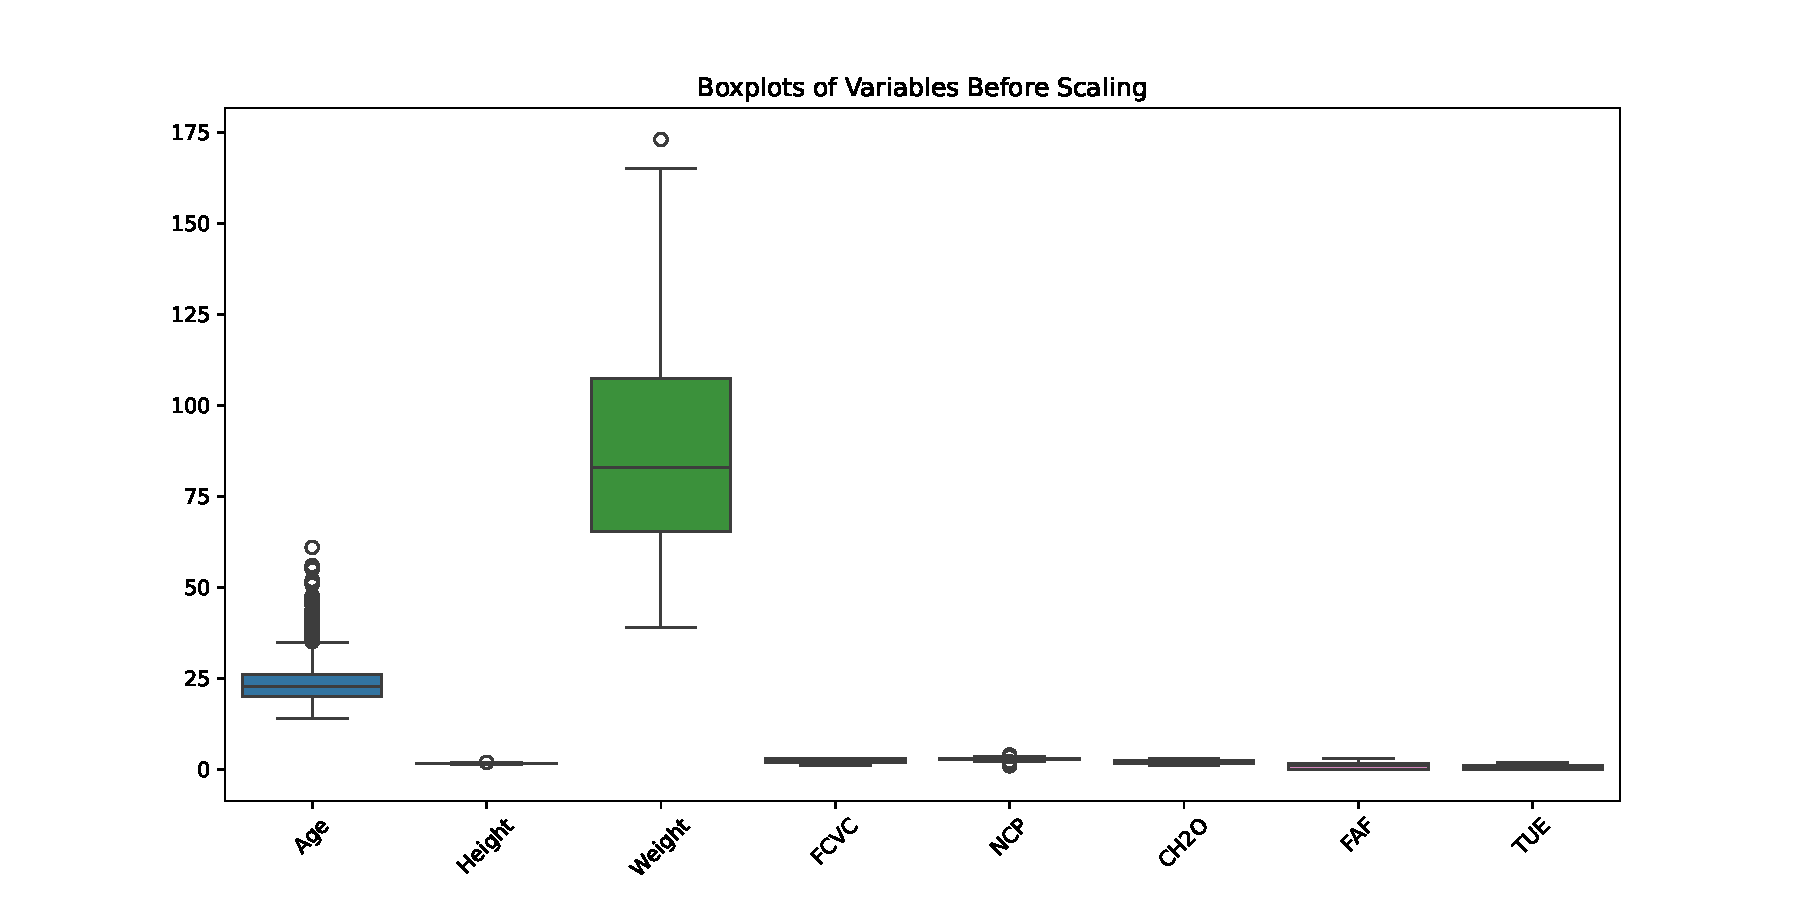
\includegraphics[width=\textwidth]{boxplots_prescale.pdf}
\caption{Boxplots of the dataset's variables before scaling}
\label{fig:boxplots_prescale}
\end{figure}

Finally, Principal Component Analysis has been used to reduce dimensionality. PCA transforms data with potentially correlated variables into a set of uncorrelated variables called principal components, ordered by the amount of variance they capture from the original data. This reduces noise and can make it easier for methods like K-Means to identify patterns. It is particularly effective where datasets have a large number of variables and where variables are likely to be highly correlated as with obesity, height and weight in this dataset \cite{Bandyopadhyay2013}. A condition has been set for the model to use the number of components necessary to capture 95\% of the variance, which ensures the model minimises the loss of potential data patterns.

\section{K-Means: results}

Before the analysis is run, K must be determined. An Elbow plot is used to identify the optimal number of clusters, found at the 'elbow point' where additional clusters no longer significantly reduce inertia. This is used here in conjunction with a Silhouette Score which evaluates cluster cohesion and separation, with higher scores indicating clearer boundaries between clusters \cite{Geron2022}. As can be seen in \ref{fig:elbow_silhouette}, the Elbow plot suggests a change in inertia around k=4, which is also the highest silhouette score, making 4 the best option. 

\begin{figure}[!h]
    \centering
    \begin{subfigure}[b]{0.8\textwidth}
        \centering
        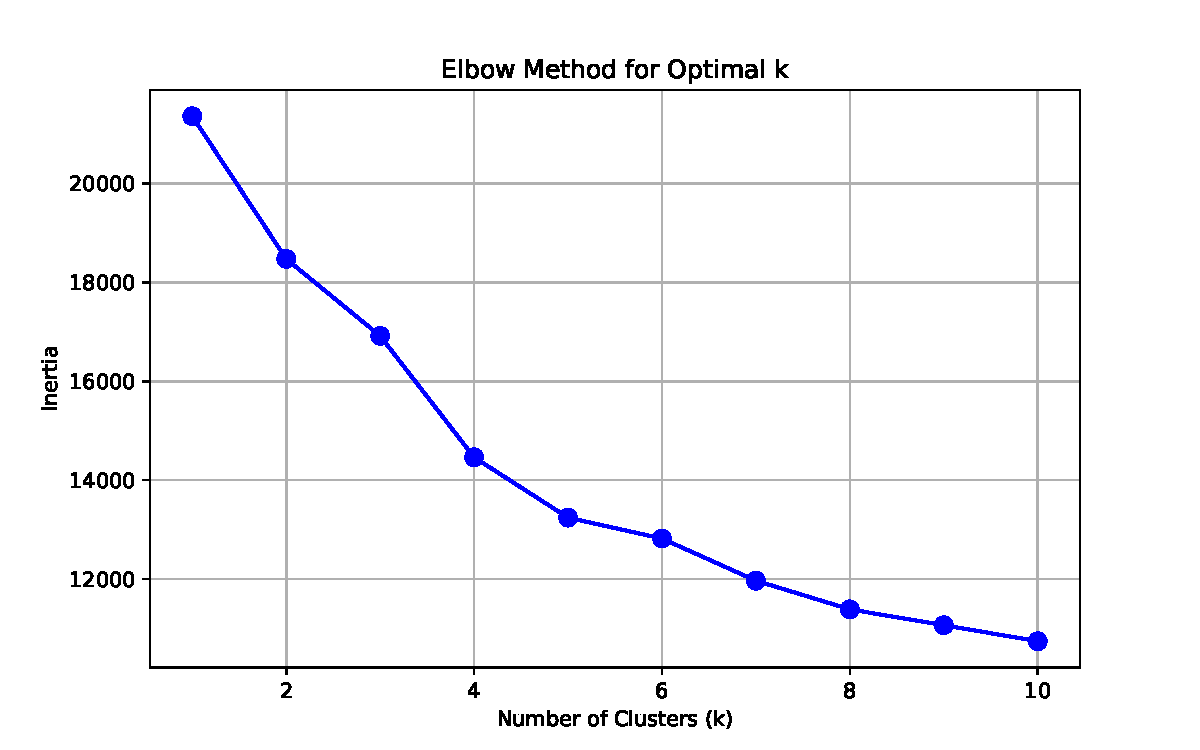
\includegraphics[width=\textwidth]{elbow.pdf}
        \label{fig:elbow}
    \end{subfigure}
    \hfill
    \begin{subfigure}[b]{0.8\textwidth}
        \centering
        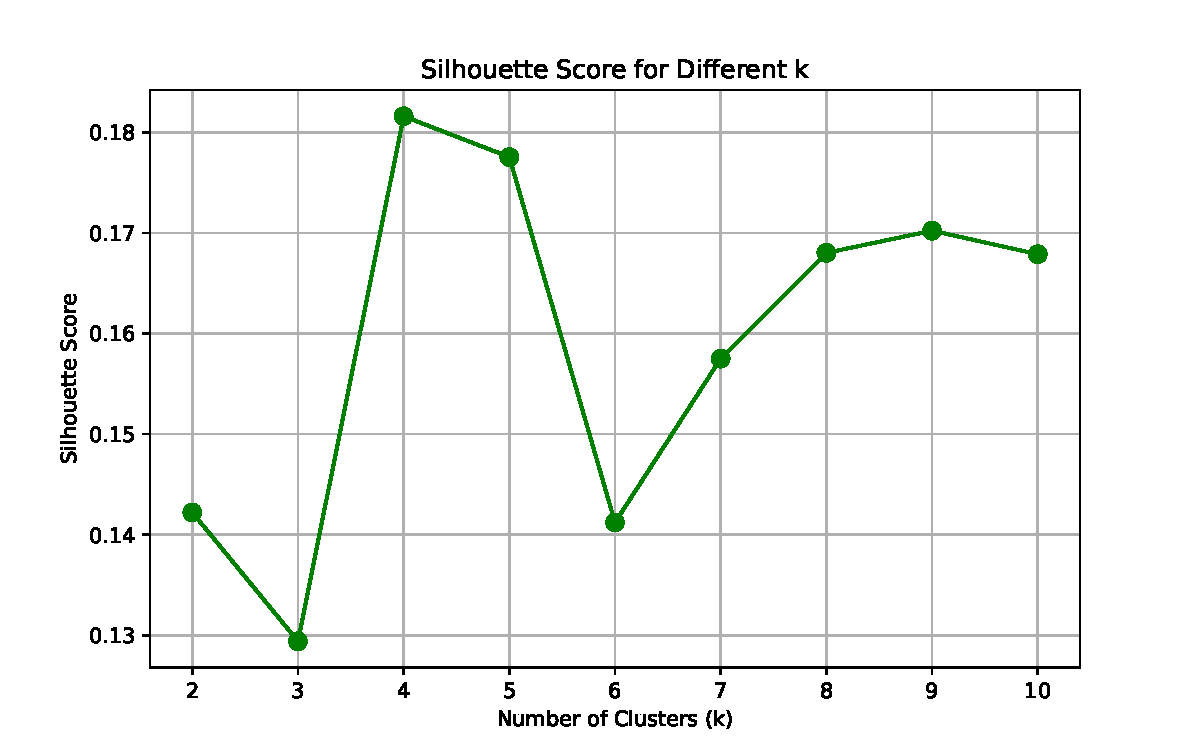
\includegraphics[width=\textwidth]{silhouette.pdf}
        \label{fig:silhouette}
    \end{subfigure}
    \caption{Comparison of Elbow Method and Silhouette Score}
    \label{fig:elbow_silhouette}
\end{figure}

The K-Means analysis was therefore run with k=4. The output cross-tabulated with the obesity categories is shown in \ref{fig:obesity_clusters}, which shows Cluster 0 is most strongly associated with Overweight Level 1, Cluster 1 with Normal Weight, Cluster 2 with Obesity Type III and Cluster 3 with Overweight Level II. The association between Cluster 2 and the highest level of obesity is particularly strong, indicating that analysis has identified a grouping with significant obesity risk. To better understand what characterises each group, \ref{tab:strongest_relationships_minipage} shows the five highest absolute mean values for variables in each cluster, excluding height and weight as the determinants of obesity rates in order to focus in on demographic and lifestyle factors.

Cluster 0 is characterised by few meals but frequent snacking, use of public transport and some prevalence of family obesity. For Cluster 1, frequency of snacking is an even more significant driver, and is coupled with high calorie food consumption. In Cluster 2 the most significant variables are family history and consumption of high calorie food, suggesting both genetic risk and unhealthy eating habits. Frequent snacking also appears and vegetable consumption is also in the top five most significant variables. Finally, in Cluster 3 age is the dominant factor, though family history remains influential, as do high calorie food consumption and frequent snacking. Assessing clusters as a whole, public transport appears frequently, though as addressed earlier in this study, that may reflect the fact that few respondents use alternative methods of transport.

In the next section, supervised analysis is used to generate further insights from the data, before the findings from both analyses are considered in the Discussion section. 

\begin{figure}[h]
    \centering
    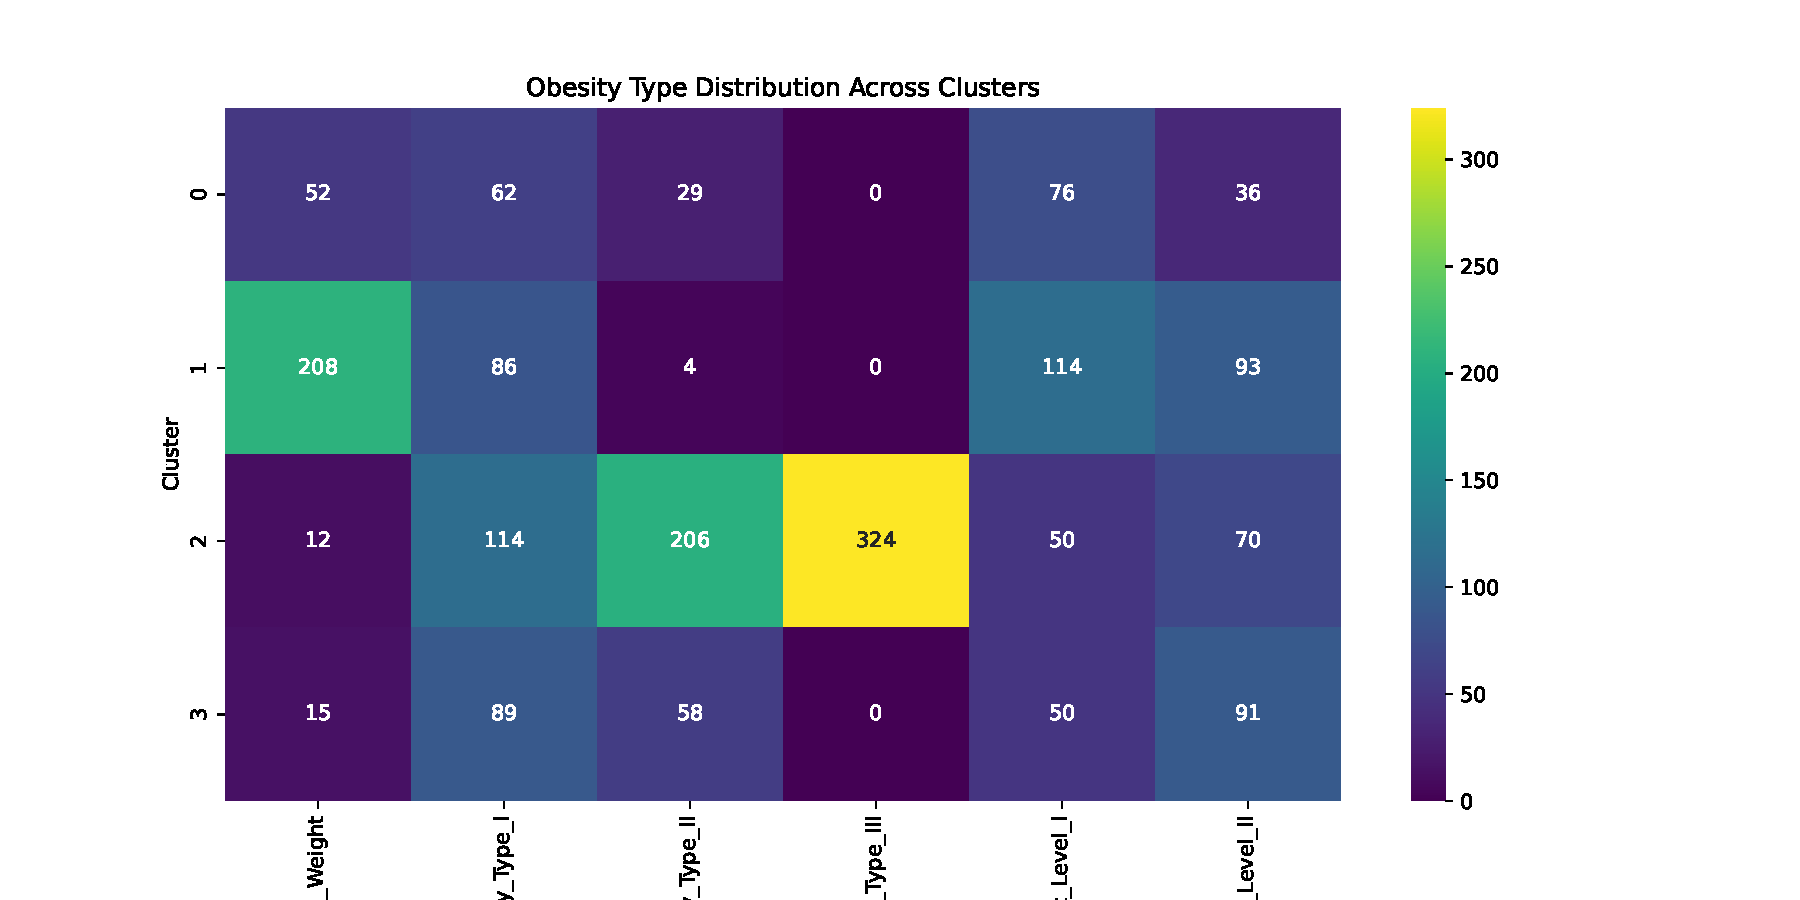
\includegraphics[width=1\textwidth]{obesity_clusters.pdf}
    \caption{Obesity Category Distribution Across Clusters}
    \label{fig:obesity_clusters}
\end{figure}

\begin{table}[h]
\centering
\caption{Top 5 Strongest Relationships per Cluster (Excluding Height, Weight, and Obesity Categories) with Strength Values}
\label{tab:strongest_relationships_minipage}

% ----------- First Row: Cluster 0 and Cluster 1 -----------
\begin{minipage}[t]{0.48\textwidth}
\centering
\caption*{\textbf{Cluster 0}}
\renewcommand{\arraystretch}{1.2}
\begin{tabularx}{\textwidth}{lXr}
\hline
\textbf{Rank} & \textbf{Feature} & \textbf{Strength} \\
\hline
1 & NCP & -1.937 \\
2 & CAEC & 1.110 \\
3 & FAVC & 0.851 \\
4 & Public Transport & 0.929 \\
5 & Family History & 0.640 \\
\hline
\end{tabularx}
\end{minipage}
\hfill
\begin{minipage}[t]{0.48\textwidth}
\centering
\caption*{\textbf{Cluster 1}}
\renewcommand{\arraystretch}{1.2}
\begin{tabularx}{\textwidth}{lXr}
\hline
\textbf{Rank} & \textbf{Feature} & \textbf{Strength} \\
\hline
1 & CAEC & 1.291 \\
2 & Public Transport & 0.812 \\
3 & FAVC & 0.793 \\
4 & NCP & 0.562 \\
5 & Family History & 0.671 \\
\hline
\end{tabularx}
\end{minipage}

% ----------- Second Row: Cluster 2 and Cluster 3 -----------
\begin{minipage}[t]{0.48\textwidth}
\centering
\caption*{\textbf{Cluster 2}}
\renewcommand{\arraystretch}{1.2}
\begin{tabularx}{\textwidth}{lXr}
\hline
\textbf{Rank} & \textbf{Feature} & \textbf{Strength} \\
\hline
1 & Family History & 0.980 \\
2 & FAVC & 0.969 \\
3 & CAEC & 1.043 \\
4 & Public Transport & 0.852 \\
5 & FCVC & 0.338 \\
\hline
\end{tabularx}
\end{minipage}
\hfill
\begin{minipage}[t]{0.48\textwidth}
\centering
\caption*{\textbf{Cluster 3}}
\renewcommand{\arraystretch}{1.2}
\begin{tabularx}{\textwidth}{lXr}
\hline
\textbf{Rank} & \textbf{Feature} & \textbf{Strength} \\
\hline
1 & Age & 1.906 \\
2 & Family History & 0.925 \\
3 & FAVC & 0.912 \\
4 & CAEC & 1.069 \\
5 & Public Transport & 0.154 \\
\hline
\end{tabularx}
\end{minipage}
\end{table}




\chapter{Supervised Analysis}
%!TEX root = CS818_assessment.tex
Supervised learning is a machine learning technique that uses labelled data to build predictive models. Decision tree analysis is one such supervised method, whereby an algorithm learns a sequence of decision rules to classify or predict outcomes based on input features. Decision trees work by iteratively partitioning a dataset, using a predictor variable and a criterion such as variance reduction as the basis for determining where to split the data. This process continues until a stopping criterion such as a maximum number of splits is reached \cite{Geron2022}. 

Similar to cluster analysis, decision tree analysis can simultaneously evaluate multiple variables. However, whilst K-Means analysis has been used to uncover latent groupings in the data, a decision tree will instead permit identification of key predictors. This can further refine our understanding of obesity risk's key drivers and their interactions.

\section{Decision Tree Analysis: results}

The analysis was run three times. First, it was completed for the full dataset. As can be seen in \ref{tab:decision_tree}, this achieved a strong accuracy score of 0.93, however the most important feature by a significant margin was 'Weight', followed by 'Height'. Given that weight is the primary determinant of BMI, it is dominating the model and overshadowing the potential predictive power of other factors. For the second run, 'Height' and 'Weight' were excluded to reduce the impact of body-measurement data on the results. Similarly, 'Age' and 'Gender' were excluded to focus specifically on lifestyle factors. The interplay between demographic features and obesity can be instructive for identifying high-risk groups. However, in focusing in on lifestyle factors, the analysis may identify behaviours that are within individuals' power to change. This model achieved an accuracy of 0.75, and the clusters were identified as the most important feature. The third and final run removed clusters to focus solely on lifestyle factors, and achieved an accuracy of 0.71. Such a small decline in accuracy indicates that whilst the clusters have helped identify groupings in the data, they do not have significant predictive power.

\begin{table}[htbp]
    \centering
    \caption{Comparison of Decision Tree Runs: Accuracy and Top 5 Features}
    \label{tab:decision_tree}
    
    % Run 1
    \begin{subtable}[t]{0.25\textwidth}
        \centering
        \caption{Run 1: 0.93}
        \begin{tabular}{ll}
            \toprule
            Feature & Imp \\
            \midrule
            Weight & 0.555 \\
            Height & 0.169 \\
            FCVC & 0.146 \\
            Age & 0.030 \\
            FAVC & 0.024 \\
            \bottomrule
        \end{tabular}
    \end{subtable}
    \hfill
    % Run 2
    \begin{subtable}[t]{0.25\textwidth}
        \centering
        \caption{Run 2: 0.75}
        \begin{tabular}{ll}
            \toprule
            Feature & Imp \\
            \midrule
            Cluster & 0.196 \\
            FCVC & 0.149 \\
            TUE & 0.097 \\
            FAF & 0.097 \\
            NCP & 0.096 \\
            \bottomrule
        \end{tabular}
    \end{subtable}
    \hfill
    % Run 3
    \begin{subtable}[t]{0.25\textwidth}
        \centering
        \caption{Run 3: 0.71}
        \begin{tabular}{ll}
            \toprule
            Feature & Imp \\
            \midrule
            TUE & 0.158 \\
            FCVC & 0.154 \\
            CH20 & 0.128 \\
            NCP & 0.111 \\
            FAF & 0.100 \\
            \bottomrule
        \end{tabular}
    \end{subtable}

\end{table}

The full list of variables and their importance in this final run is captured in \ref{fig:feature_importance}, and shows the most significant features were TUE (time on devices) and FCVC (vegetable consumption). The effectiveness of the model itself is captured in the classification report in table \ref{tab:classification_report}. A decision was made not to set a max depth for the decision tree to allow the model to capture more complex patterns. However, this can also increase the risk of overfitting. Looking at the classification report, while some classes, notably Obesity Type I, show lower recall and F1-scores, the overall balanced performance - with an accuracy of 0.71 and similar macro and weighted averages — suggests the model is not severely overfitting. This gives confidence that the model is capturing meaningful patterns across most classes rather than just memorizing the training data. 

\begin{table}[h]
\centering
\begin{tabular}{lcccc}
\toprule
\textbf{Class} & \textbf{Precision} & \textbf{Recall} & \textbf{F1-score} & \textbf{Support} \\
\midrule
Normal\_Weight      & 0.75 & 0.77 & 0.76 & 179 \\
Obesity\_Type\_I     & 0.64 & 0.58 & 0.61 & 102 \\
Obesity\_Type\_II    & 0.77 & 0.83 & 0.80 & 88  \\
Obesity\_Type\_III   & 0.94 & 0.98 & 0.96 & 98  \\
Overweight\_Level\_I & 0.52 & 0.48 & 0.50 & 88  \\
Overweight\_Level\_II& 0.53 & 0.54 & 0.54 & 79  \\
\midrule
Accuracy            &      &      & 0.71 & 634 \\
Macro Avg           & 0.69 & 0.70 & 0.69 & 634 \\
Weighted Avg        & 0.71 & 0.71 & 0.71 & 634 \\
\bottomrule
\end{tabular}
\caption{Classification Report}
\label{tab:classification_report}
\end{table}

\begin{figure}[h]
    \centering
    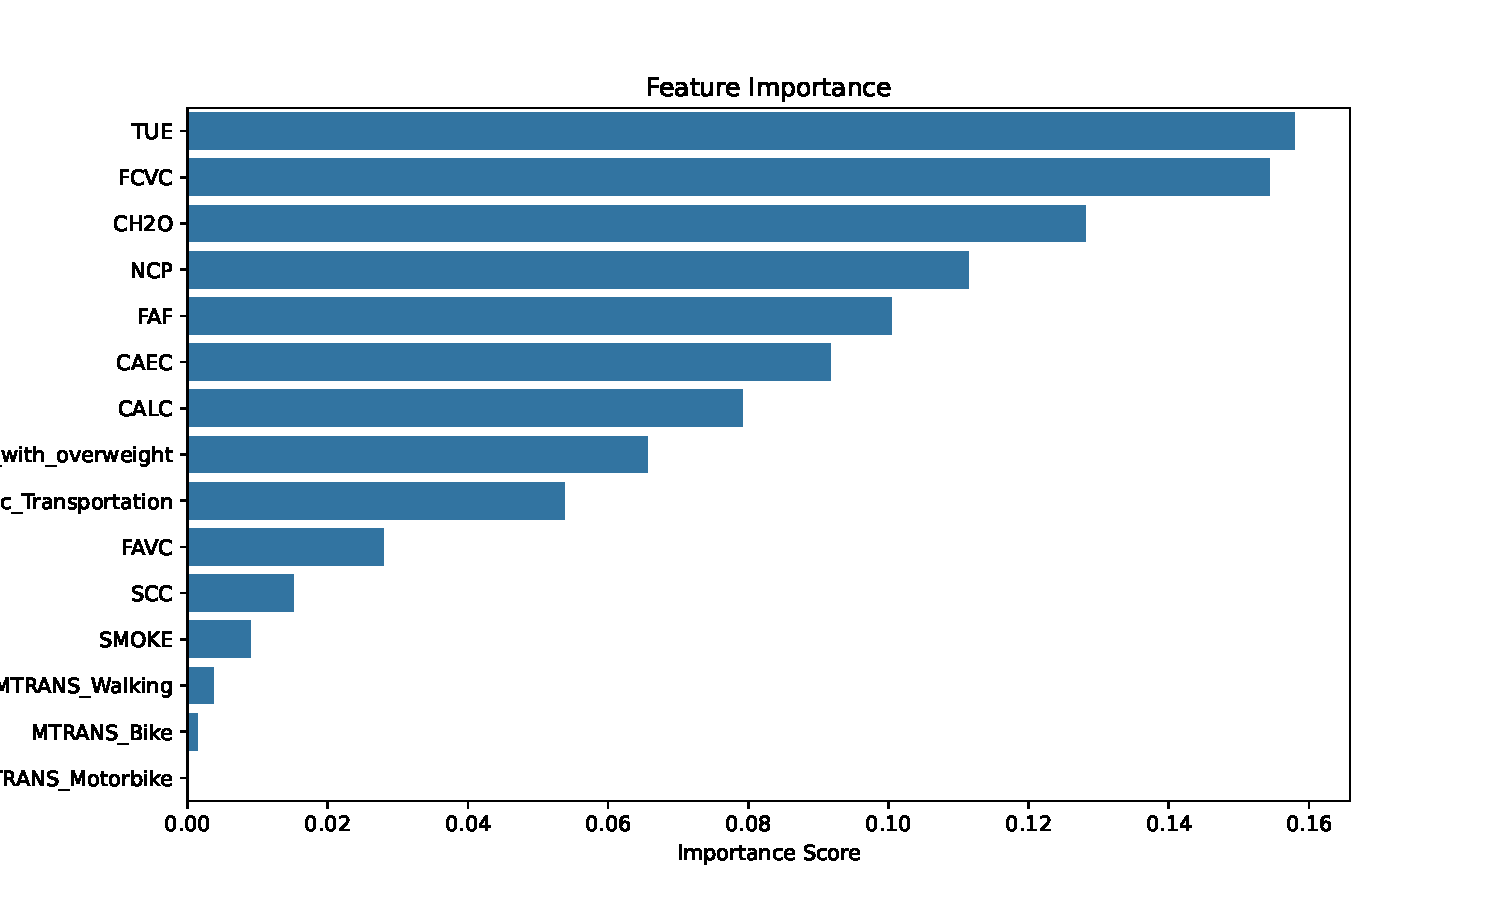
\includegraphics[width=1\textwidth]{feature_importance.pdf}
    \caption{Feature Importance Plot for Final Decision Tree}
    \label{fig:feature_importance}
\end{figure}




\chapter{Discussion}
%!TEX root = CS818_assessment.tex
The cluster analysis showed that the cluster associated with the highest obesity group was characterised by a family history of obesity, use of public transport, as well as frequent snacking and consumption of high calorie food. However, the cluster most strongly linked to normal weight also had strong associations with snacking and high calorie food, underscoring the high variability of diet's impact on individuals. It also suggests that whilst dietary habits play a significant role in obesity risk, their influence could be moderated in normal weight groups by other factors such as physical activity levels or a hereditary predisposition towards a certain weight. It could also be indicative of factors not well captured in the data such as variance in individuals' metabolic response to foods, which may allow some individuals to maintain a healthy weight despite a high caloric intake \cite{Piaggi2019}. Any cause-effect relationships therefore appear to be obscured by layers of behavioural, demographic and  genetic or hereditary interactions. These relationships were further interrogated with the decision-tree. 

Whilst the full decision-tree has too many branches to be easily interpretable, a look at the initial branches in figure \ref{fig:decision_tree}, which has a max branch depth of 3, highlights the model's most important features.

\begin{sidewaysfigure}
    \centering
    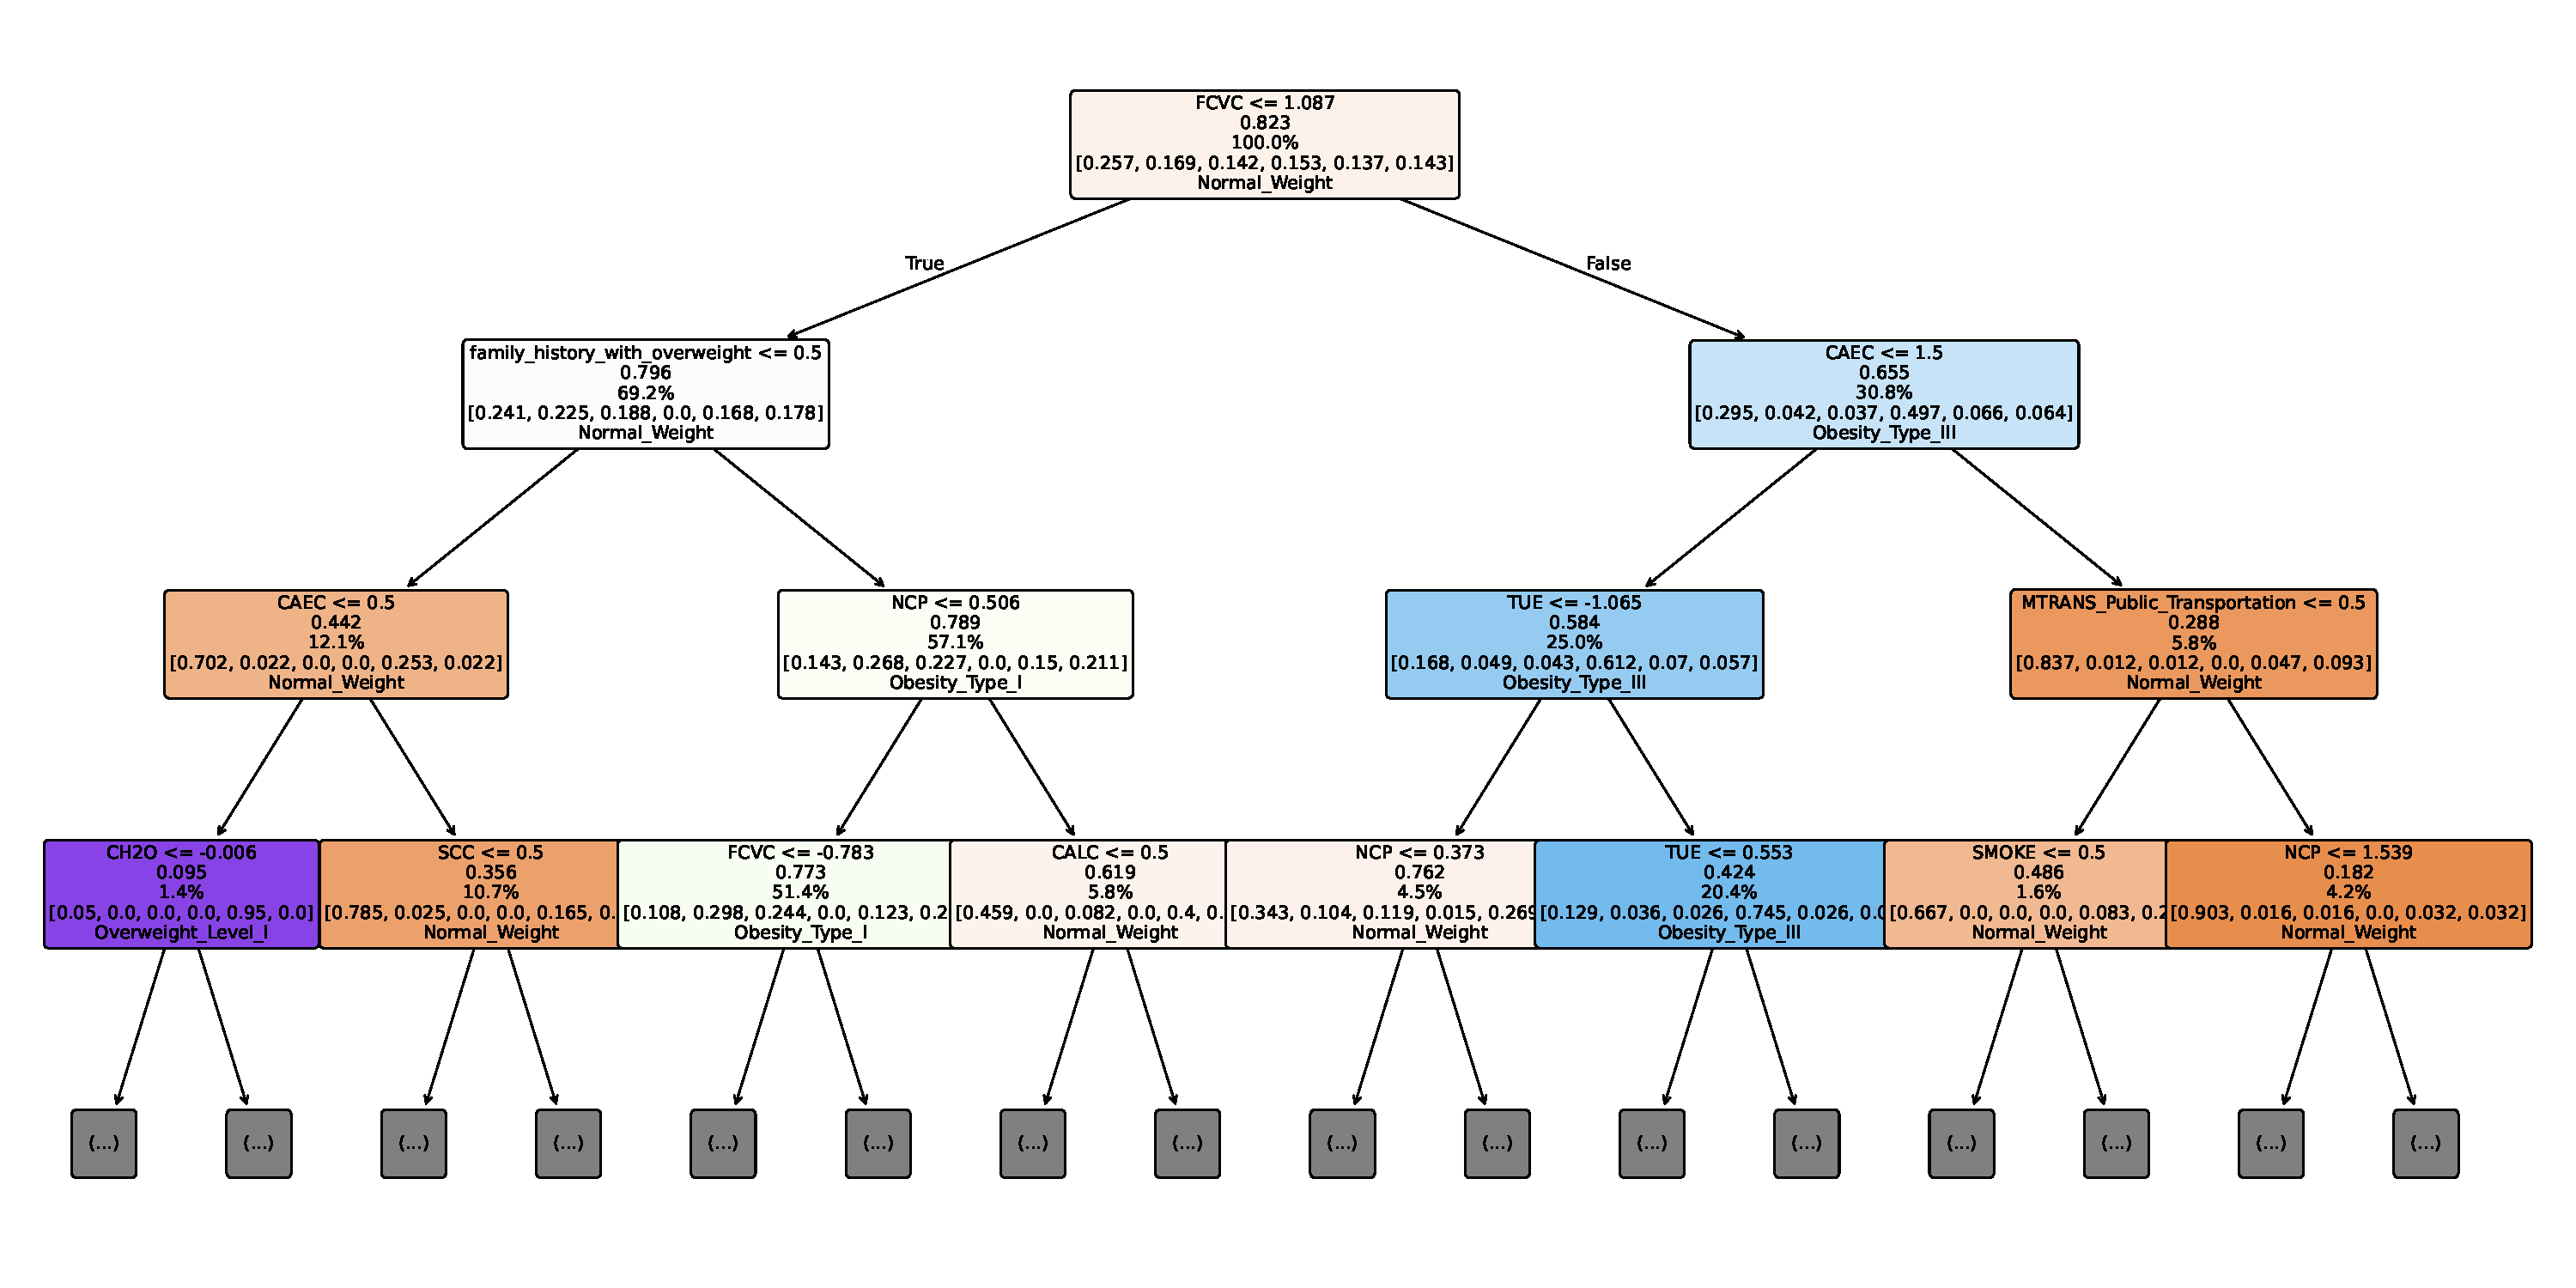
\includegraphics[width=\textwidth]{decision_tree.pdf} % Replace with your image
    \caption{Decision tree with a max depth of 3}
    \label{fig:decision_tree}
\end{sidewaysfigure}

This identifies some surprising relationships. For example, lower vegetable consumption appears to be generally associated with higher weight classes, however higher vegetable consumption together with more time spent on devices is linked to Obesity Type III, the group with the highest BMI. The relationship between FCVC and BMI was picked up in the initial exploratory analysis, but the decision-tree permits a deeper dive into the association, in particular by highlighting the influence of TUE. Whilst vegetable consumption may be predictive of obesity rates, the relationship here is not linear or omnidirectional. Instead, it is highly context dependent. The fact that high vegetable consumption appears to be generally linked to normal weight suggests it may have a protective effect in line with existing literature \cite{Nour2018}, however this impact may then be cancelled out by low physical activity. There may also be other factors not captured by the model that influence the high consumption amongst the highest BMI individuals. For example, people who are conscious of their weight may increase vegetable intake given public health messaging around the benefits, or it could reflect a 'social desirability bias'. This is where individuals are inclined to self-report socially desirable behaviours, which would lead them to over-report healthy behaviours and under-report unhealthy ones \cite{Hebert1995}. Seeking a better understanding of this relationship would be an interesting avenue for future research, given the extent to which it contradicts consensus in the literature. 


\chapter{Conclusion}
%!TEX root = CS818_assessment.tex
This analysis reconfirms that obesity risk is not monolithic, but rather varies greatly across different subpopulations defined by both lifestyle and demographic factors. Whilst traditional metrics remain critical, a richer understanding of obesity and its multifactorial nature is achieved when more sophisticated statistical tools are used. The findings of the study also suggest some potential areas of focus for public health interventions, notably physical activity. Use of public transport and high screentime were two of the study's most significant variables relating to obesity risk, with these factors even potentially nullifying some of the benefits of other healthy behaviours. One potential intervention could therefore be promoting active transport. The initial exploratory analysis showed respondents overwhelmingly rely on public transport, and to a lesser degree automobiles. The low prevalence of cycling and walking at present suggests this could be an impactful way to reduce overall sedentary time in these countries. 

Despite these strengths, there are also a number of weaknesses and limitations in the research. The analysis is based on a rich dataset which is nevertheless made up primarily of synthetic data, and the utility and generalisability of the data is dependent on the strength of the data generation methods used. Finally, this study is cross-sectional, examining data at a single point in time. The variables studied here and their relationships may vary over time, which could impact the conclusions drawn. Whilst particular relationships, such as that between high vegetable consumption and the highest BMI, have already been highlighted as potentially useful avenues for future research, further studies should also include longitudinal studies that observe how these factors interact over extended time-frames. Similarly, rerunning the analysis on other datasets could further validate the findings, improve the generalisability of results, and address some of the data quality concerns outlined above. In this way, we can continue to build on the analysis set out here and shed further light on a complex and multifaceted public health issue. 


\chapter{Appendix}
\section{Development environment}
All analyses were implemented in Python 3.12, using Jupyter Notebooks and Neovim to write and test the code. The paper was written in Neovim using the VimTex plugin.  
\section{Supplementary figures}
%!TEX root = CS818_assessment.tex

\begin{figure}[htbp]
    \centering
    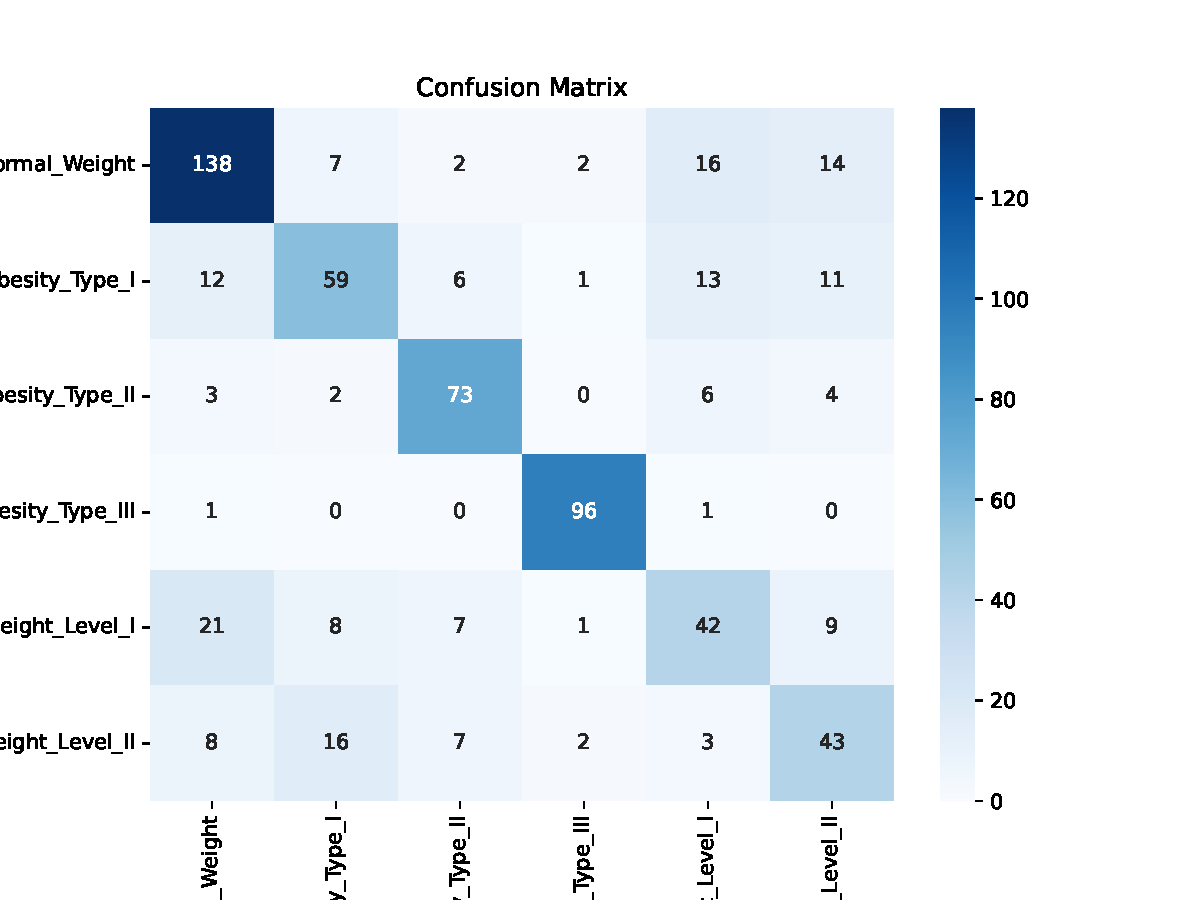
\includegraphics[width=0.7\textwidth]{confusion_matrix.pdf}
    \caption{Confusion Matrix for Final Decision Tree}
    \label{fig:confusion_matrix}
\end{figure}

\begin{figure}[!h]
    \centering
    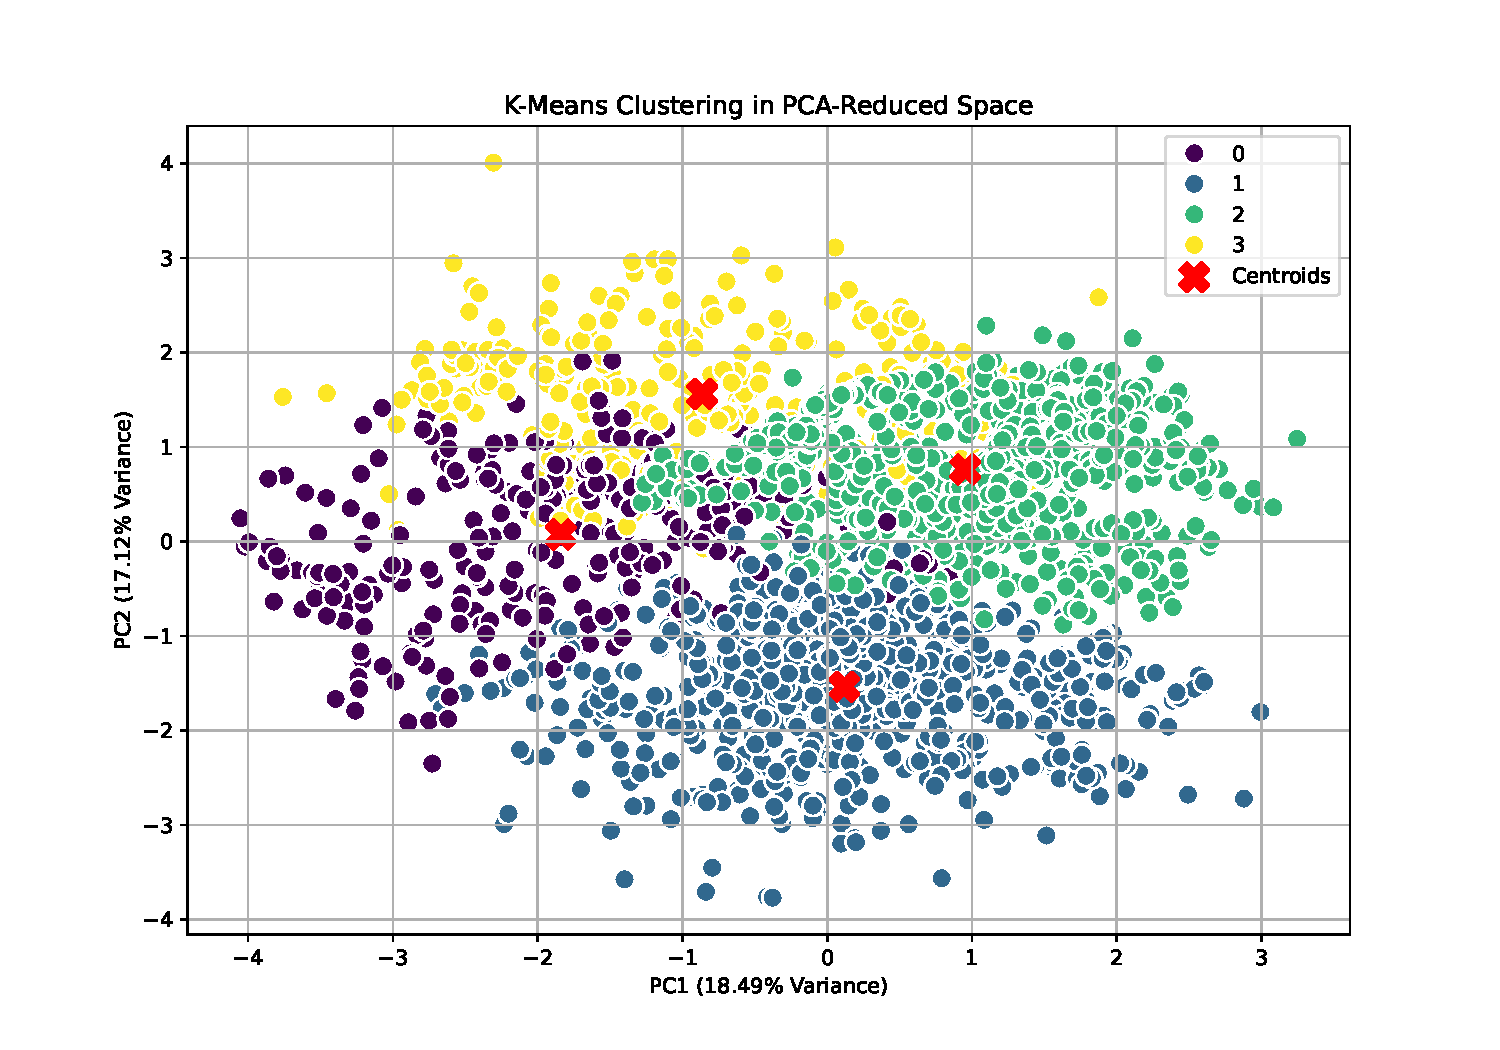
\includegraphics[width=0.8\textwidth]{kmeans_pca_reduced.pdf}
    \caption{K-Means Clustering in PCA-Reduced Space}
    \label{fig:kmeans_pca}
\end{figure}




\printbibliography

\end{document}
